\section{Identification of Metal Foils by their Absorption Edges}
\label{sec:identify}

In the following section, we are going to identify an unknown metal foil due to its absorption edges. The used setup is described in Chapter \ref{sec:SetupAbsorb}.
The setup is able to measure the transmitted intensity in regard to a diffraction angle. The measured angle $\omega = 2\Theta$ can be varied from $5.0^\circ \leq \, \omega \, \leq 51.0^\circ$ with a step width of $0.1^\circ$. In the beam path, we placed three foils marked with an index 2, 3, 4 of thickness $d_\mathrm{f} = 2.5\cdot10^{-5}$\,m. A reference measurement was performed as well.

\subsection{Calibration of the Device}
\label{sub:calibration}

% m = 0.99621756 +/- 0.00215493
% t = 0.2838616 +/- 0.034687

% Corr Theta 0.2491746012633316 

First step is to calibrate the machine to evaluate the correct data from the measurement. For this we use the known characteristic radiation of our Tungsten anode. The sharp peaks should be visible in the X-Ray intensity spectrum if they fulfill the Bragg condition

\begin{gather}
    2 d \sin{\omega} = n \lambda~,
    \label{eq:bragg}
\end{gather}

with $\omega$ being same angle mentioned above, $ \lambda $ being the wavelength of the spectrum, $n$ the oder of diffraction and $d$ being the grid plane spacing. For the cubic $\mathrm{CaF}_2$ crystal, which is used in this experiment as reference, the grid plane distance can be calculated as

\begin{equation}
    d_{hkl} = \sqrt{\frac{a^2}{h^2+k^2+l^2}}~,
\end{equation}

with $(hkl) = (220) $ being the Laue indexes and $a = (5.463 \pm 0.001)$\,\AA. Therefore, $d = (1.9314 \pm 0.0004)$\,\AA~in this geometry. Since the errors are very small, they will be neglected for the rest of the evaluation. To calculate the angle of Equation (\ref{eq:bragg}) gets rearanged for the angle $\omega$ as following

\begin{gather}
    \omega = \arcsin\left(\frac{n \lambda}{2 d}\right)~.
    \label{eq:angle}
\end{gather}

Assuming the dominant peaks for lower angle are peaks due to the first order of the diffraction ($n = 1$), we correlate those with the known peaks from Ref. \citenum{Anleitung}. The smaller one are correlated to the second order of diffraction ($n = 2$). The theoretical values for the characteristic peaks of the wolfram anode are from \textit{National Institute of Standards and Technology}. Transforming the theortical peak values given in $\lambda$ into angles in our geometry $\Theta$ and taking into account their relative intensity, the peaks are identifiable as the peaks of the \textit{Lyman series}.
\bigskip
To calibrate our device, we assume linear scale with the parameters: $t$ as offset and $m$ as slope. Therefore, we 
fit a straight line to our data $\Theta_\mathrm{Data}$ plotted against the theoretical values $\Theta_\mathrm{Theo}$ for the first and second order together with the following equation
\begin{gather}
    \Theta_\mathrm{Theo} = m * \Theta_\mathrm{Data} + t~.
    \label{eq:fitLin}
\end{gather}
The fit can be seen in Fig. \ref{fig:linearFit}. Calculation yields following result
\begin{gather*}
    \boxed{m = 0.996 \pm 0.002 \qquad t = (0.284 \pm 0.035)^\circ}~.
\end{gather*}
These two parameters will be used to calibrate our device from now on. In Fig. \ref{fig:wolfram} one can see the correctness of the calibration for the frist order and second order diffraction peaks.

\begin{center}
    \captionsetup{type = figure}
    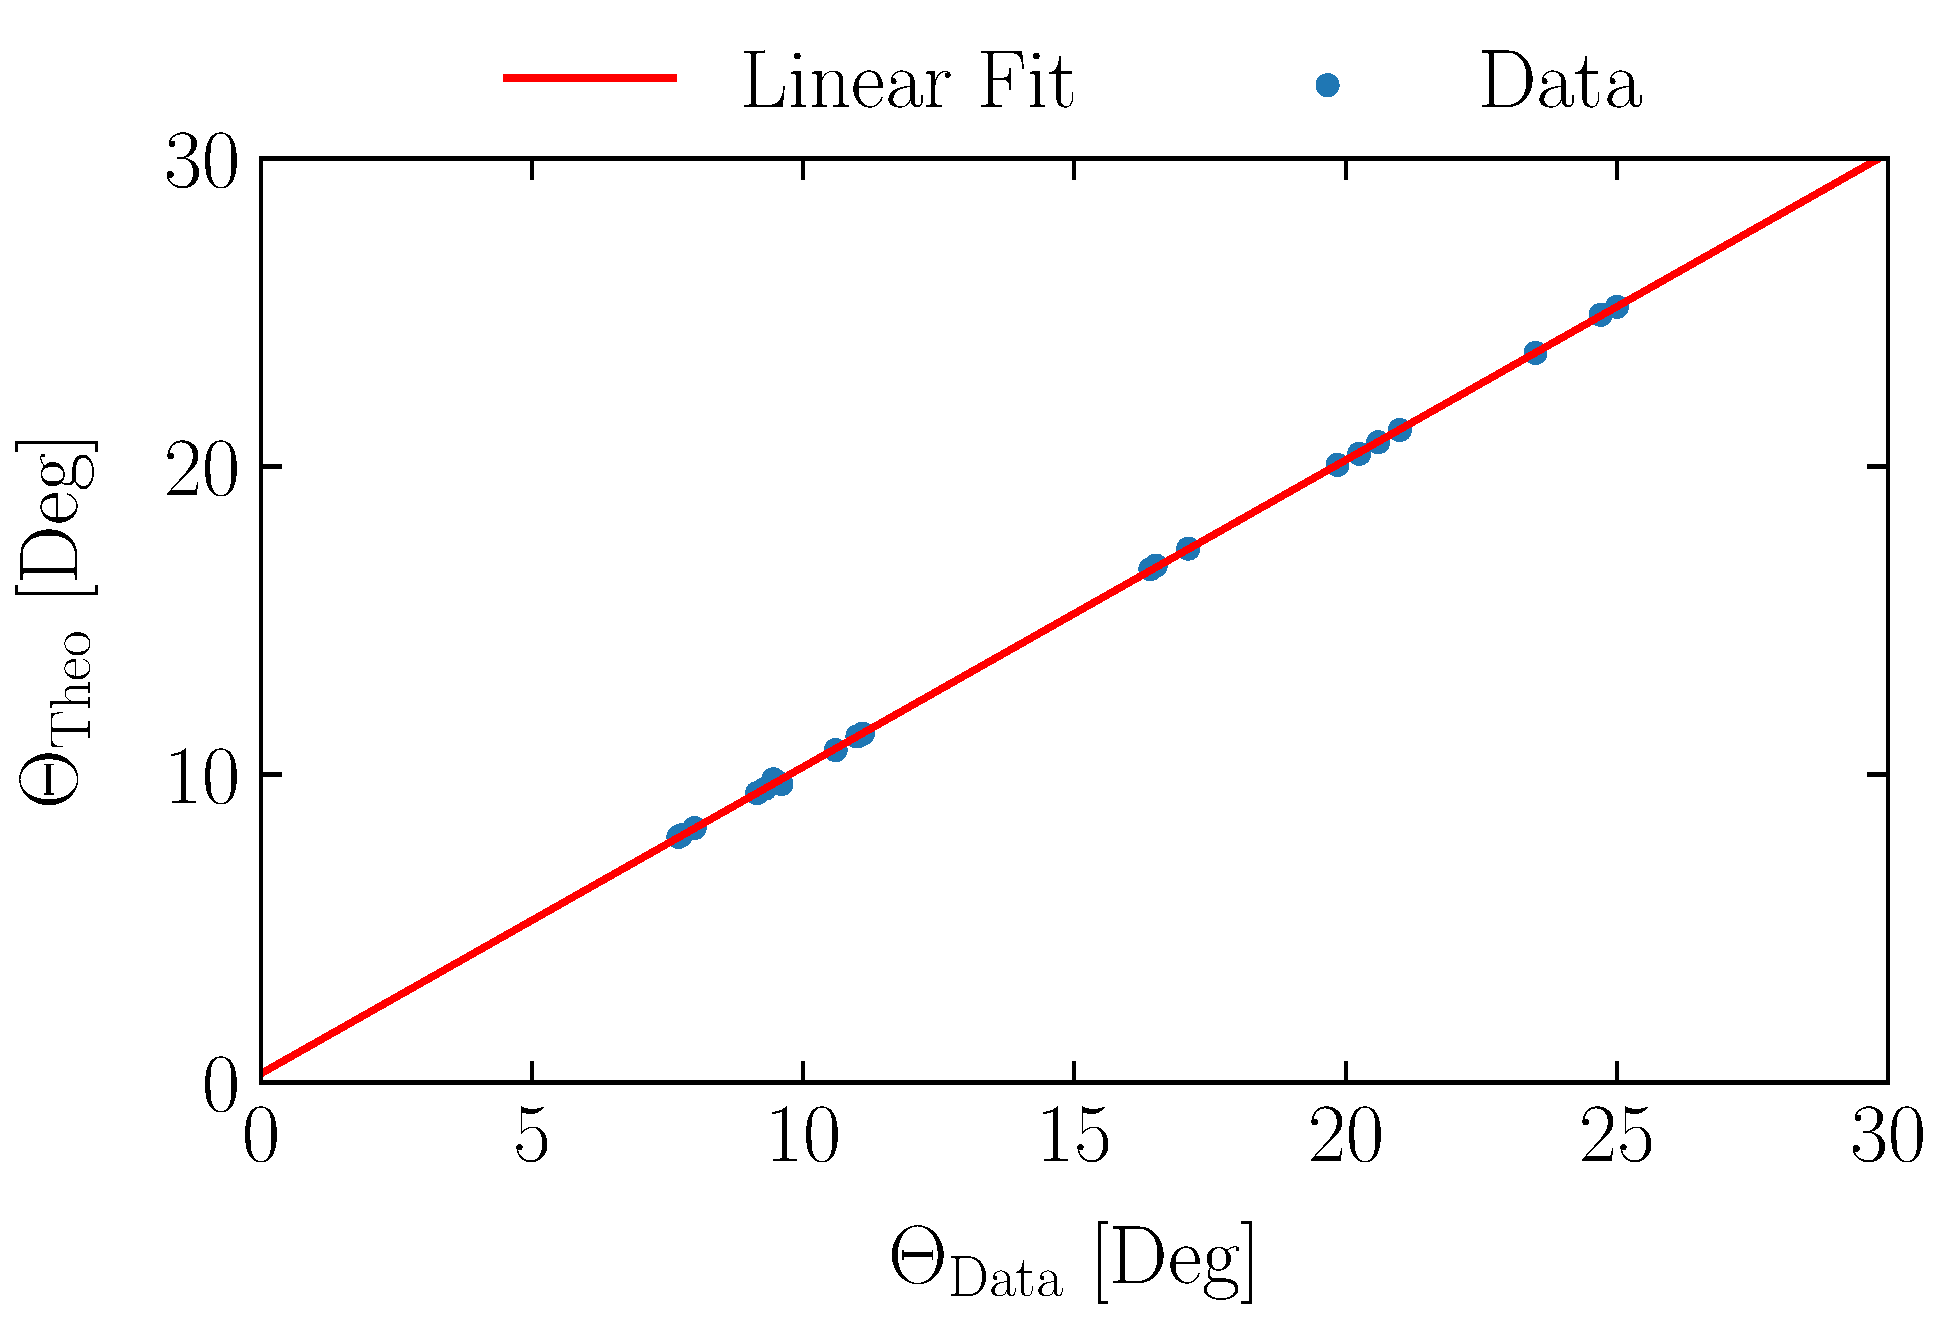
\includegraphics[width = 0.7\textwidth]{Pictures/Evaluation/41/Linear-Fit.pdf}
    \captionof{figure}{
        The extracted peaks $\Theta_\mathrm{Data}$ are compared to the theoretical values $\Theta_\mathrm{Theo}$ and are fitted with a linear fit function. Note that the fit was performed for first and second order peaks together. 
    }
    \label{fig:linearFit}
\end{center}

\begin{center}
    \begin{sidewaysfigure}
    \centering
    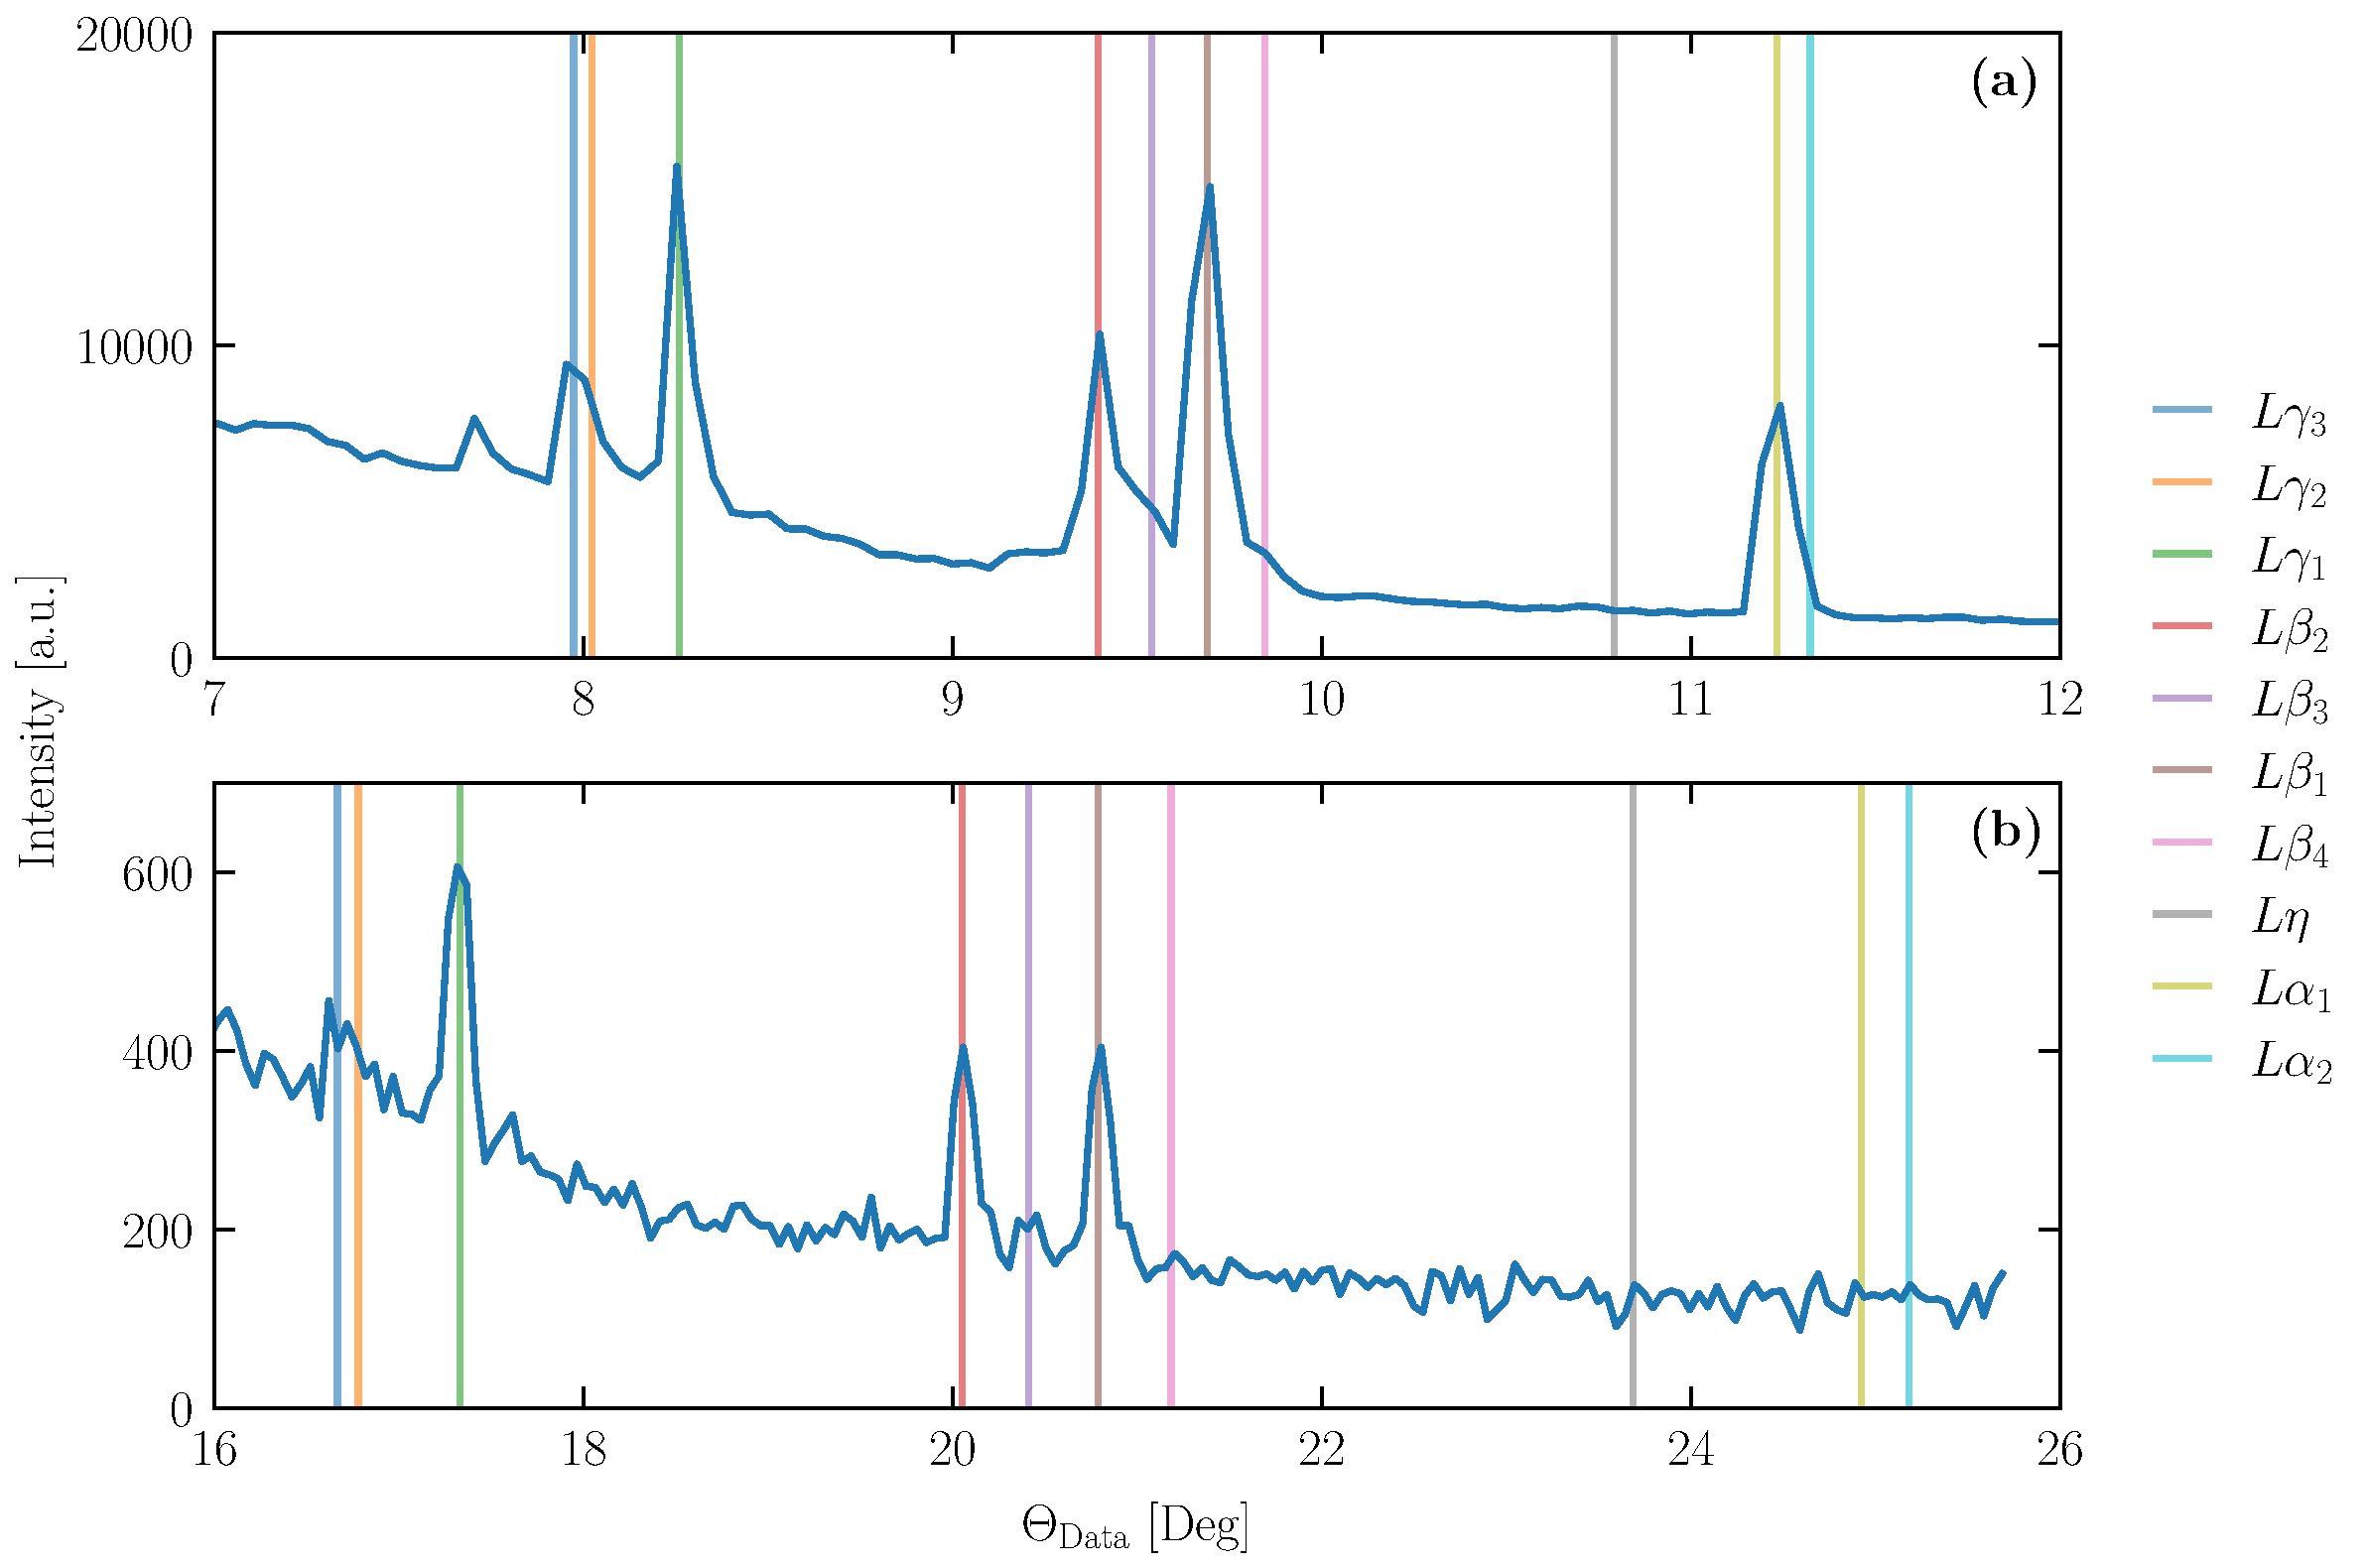
\includegraphics[width = 0.9\textheight]{Pictures/Evaluation/41/Wolfram-Spectrum.pdf}
    \caption{
        Corrected X-Ray spectrum of the device with the theortical values of the peaks named in Siegbahn notation. In (a) the peaks of first order are displayed and in (b) the peaks of second order.
    }
    \label{fig:wolfram}
    \end{sidewaysfigure}
\end{center}

\newpage

\subsection{Identification of Metal Foils}
\label{sub:identification}

In this section we want to identify the type of metal for foil 2, 3, 4. When a metal is irradiated with X-Rays, strong, irregular absorption bands become visible. These are created when the electrons exceed a certain energy form, they can interact and free electrons from lower energy levels of the atom. This leads to a sharp jump in the absorption. The mass attenuation coefficient $\mu/\rho$ is from special intrest. It can be derived from the Lambert-Beer Law and is given by
\begin{equation}
    \frac{\mu}{\rho} = \frac{1}{\rho d_\mathrm{f}}\log(\frac{I_0}{I})~,
\end{equation}
with the density $\rho$ and the thickness of the foil $d_\mathrm{f}$. The specific energy at which those jumps take place depend on the internal energetically structure of the atom, especially on the number of protons. Therefore, it is possible to distinguish the different metals. The different X-Ray absorption spectrums for each foil are shown in Fig. \ref{fig:xRay} with transfromed angle $\Theta$ into wavelength $\lambda$ under the use of Equation (\ref{eq:bragg}) with $n=1$. 

\begin{center}
    \captionsetup{type = figure}
    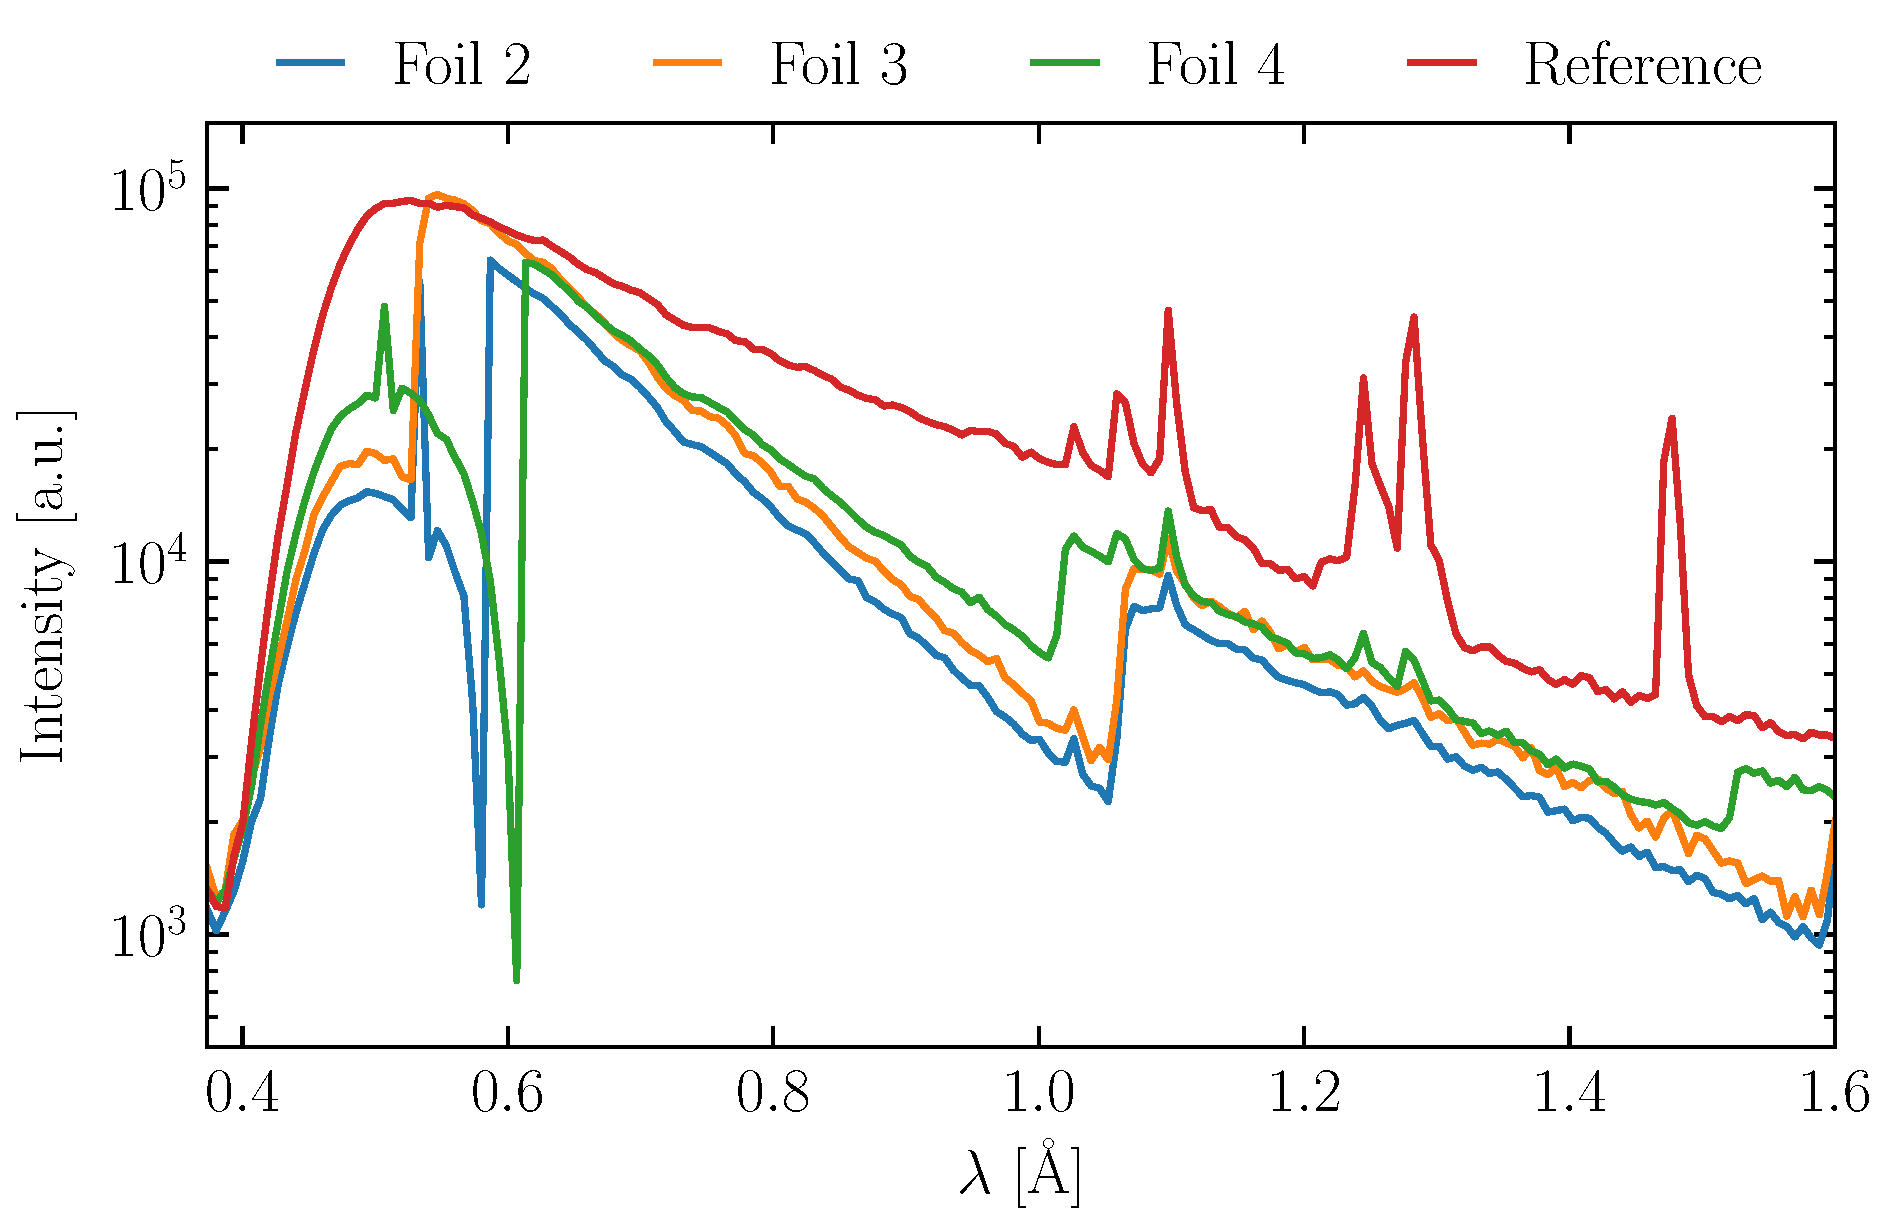
\includegraphics[width = 0.8\textwidth]{Pictures/Evaluation/41/XRay-Spectrum.pdf}
    \captionof{figure}{
        X-Ray intensity spectrum of foil 2, 3 and 4 plotted against the reference signal with logarithmic y axis. The reference signal and the signal of foil 3 was shifted in height to achieve alignments.
    }
    \label{fig:xRay}
\end{center}

A closer look at the first sharp jump in the spectrum yields following result with the comparison from the \textit{National Institute of Standards and Technology}\cite{XRayDatabase}
\begin{itemize}
    \item \textbf{Foil 2}: 0.585\,\AA~$\Rightarrow$ Pd (Palladium) (or Np (Neptunium)),
    \item \textbf{Foil 3}: 0.530\,\AA~$\Rightarrow$ Rh (Rhodium) (or Cf (Californium)) and
    \item \textbf{Foil 4}: 0.610\,\AA~$\Rightarrow$ Not exactly determinable.
\end{itemize}
In the case of foil 4 it is not clear from the database which metal foil 4 contains. In the range of the evaluated value one can only find elements which are radioactive, so we assume a measurement error occurred. The frist sharp edge of each foil is displayed in Fig. \ref{fig:foil}. For the other foils the result is also too inaccurate to determine the right metal. 
\bigskip

Since the evaluation of the first sharp jump does not yield exact results, no further evaluations will be performed.

\begin{center}
    \captionsetup{type = figure}
    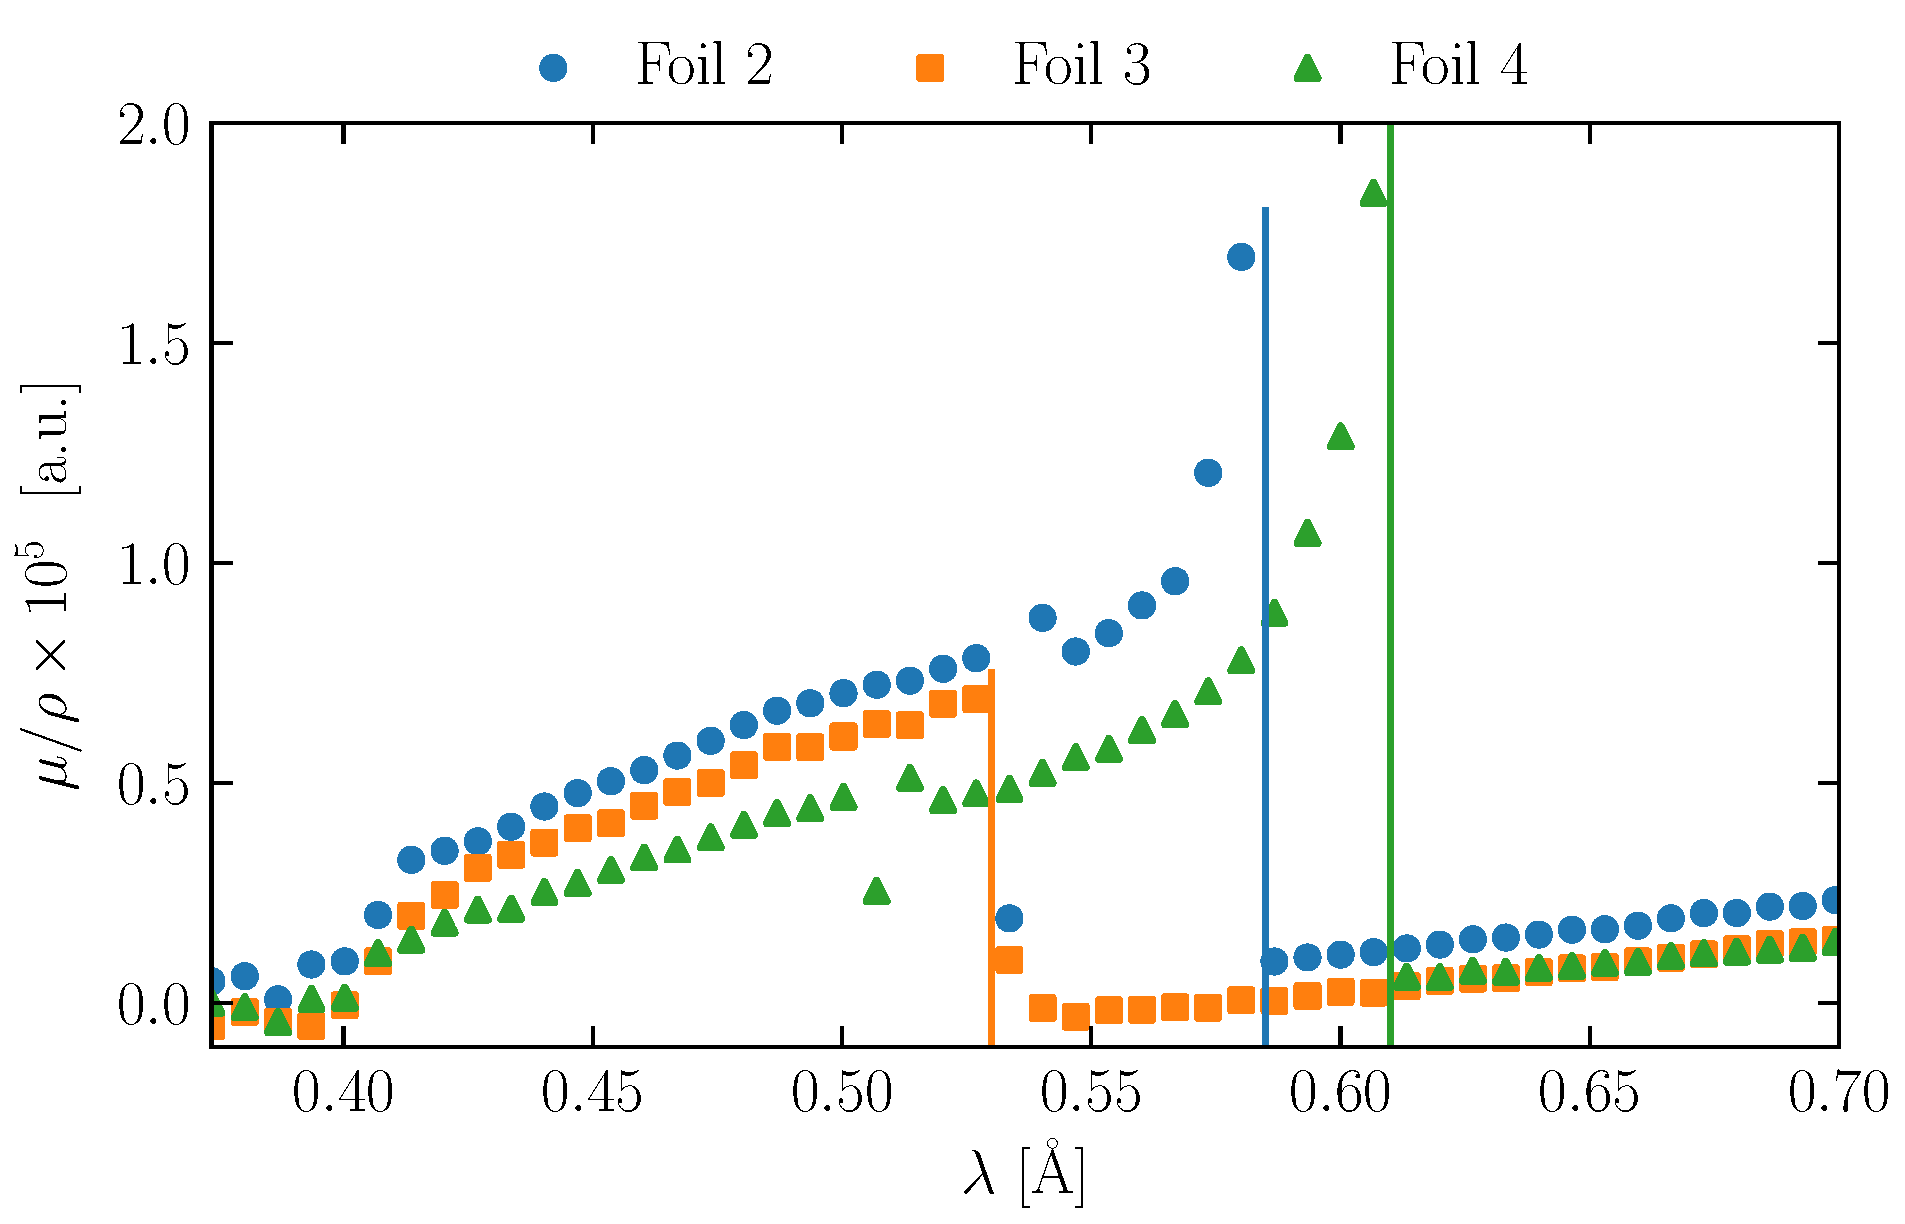
\includegraphics[width = 0.8\textwidth]{Pictures/Evaluation/41/Analysis-Foil.pdf}
    \captionof{figure}{
        The absorption takes a sharp jump for the foil 2 close to $\lambda = 0.585$\,\AA, for foil 3 close to $\lambda = 0.530$\,\AA and for foil 4 close to $\lambda = 0.610$\,\AA.
    }
    \label{fig:foil}
\end{center}